\documentclass[conference]{IEEEtran}
\usepackage{amsmath,amssymb}
\usepackage{graphicx}
\usepackage{cite}
\usepackage{url}
\usepackage{booktabs}

\title{An Educational Python Simulation of an LMS Linear Equalizer}
\author{\IEEEauthorblockN{Author One, Author Two, Author Three}
\IEEEauthorblockA{AVD612 Course Project\\
Indian Institute of Space Science and Technology\\
Replace with your team's details}}

\begin{document}
\maketitle

% COURSE REMINDER: This is a writing scaffold, not a final report.
% Rewrite explanations in your own words, verify all results from your own run,
% identify the actual contributions of each team member, and keep within six pages.

\section{Introduction}
% Write a concise introduction in your team's own words.
% Explain what an adaptive equalizer is, why multipath causes ISI, and where
% this receiver block fits in a digital communication link. Cite a textbook.

\section{Informal Explanation of the Subsystem}
% Explain the tap-delay line in plain language. Discuss the known training
% sequence and the optional decision-directed mode. Refer to the simulator's
% block diagram if your team creates one.

\section{Mathematical Model}
A symbol-spaced multipath channel can be represented as
\begin{equation}
 r[n] = \sum_{k=0}^{L-1} h[k]a[n-k] + v[n],
 \label{eq:channel}
\end{equation}
where $a[n]$ is the transmitted symbol, $h[k]$ are channel coefficients, and
$v[n]$ is additive noise. The equalizer input vector contains $M$ received
samples:
\begin{equation}
 \mathbf{x}[n] = [r[n],r[n-1],\ldots,r[n-M+1]]^T.
\end{equation}
For the complex baseband convention used in the implementation, the equalizer
output and error are
\begin{align}
 y[n] &= \mathbf{w}^H[n]\mathbf{x}[n],\\
 e[n] &= d[n]-y[n],
\end{align}
where $d[n]=a[n-D]$ is the desired symbol at decision delay $D$.
The least-mean-squares (LMS) update is
\begin{equation}
 \mathbf{w}[n+1] = \mathbf{w}[n] + \mu\mathbf{x}[n]e^*[n],
 \label{eq:lms}
\end{equation}
where $\mu$ is the step size and $^*$ denotes complex conjugation. Equation
\eqref{eq:lms} adjusts the tap weights after observing the current error. LMS
adaptive filtering is covered in standard references such as~\cite{haykin2014adaptive};
GNU Radio also documents training-based and decision-directed linear equalization~\cite{gnuradioLinearEqualizer}.
% In your own words, show the key gradient step or explain the stochastic
% gradient approximation. Do not include a derivation you cannot explain.

\section{Implementation}
% Explain the responsibilities of modulation.py, channel.py, equalizer.py,
% simulation.py, and plotting.py. State how you selected the tap count, step
% size, decision delay, training fraction, and SNR. Describe the split between
% training targets and test targets.

\section{Test Results}
% Regenerate the figures from the final version of the code. Include parameter
% settings and discuss all observed trends, including any setting where LMS did
% not improve performance. Do not claim a result without running it yourself.

\begin{table}[t]
\centering
\caption{Example measurements from the default reproducible run. Verify these values with your final run.}
\label{tab:metrics}
\begin{tabular}{lcc}
\toprule
Metric & Before LMS & After LMS \\
\midrule
BER & 0.003857 & 0.000000 \\
Normalized EVM & 0.4454 & 0.1358 \\
\bottomrule
\end{tabular}
\end{table}

\begin{figure}[t]
\centering
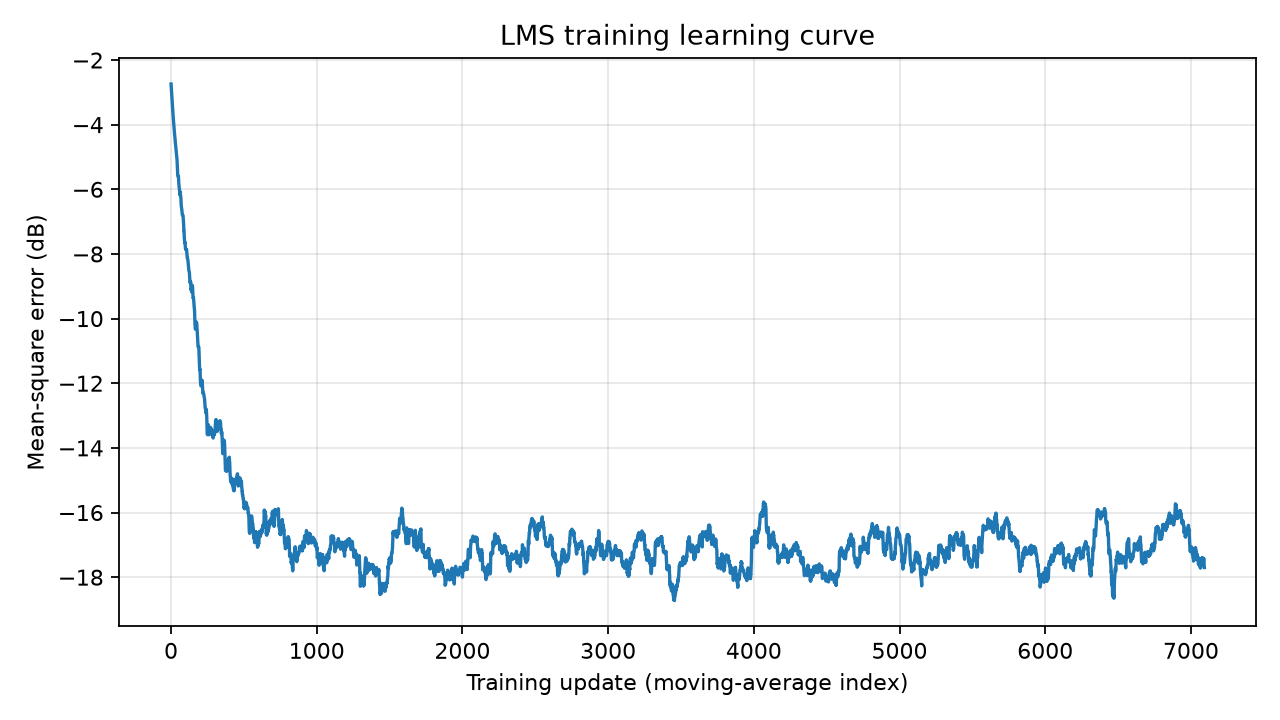
\includegraphics[width=0.98\columnwidth]{../results/learning_curve.png}
\caption{Training error averaged over a short sliding window. Replace or retain only after inspecting the final experiment.}
\label{fig:learning}
\end{figure}

\begin{figure}[t]
\centering
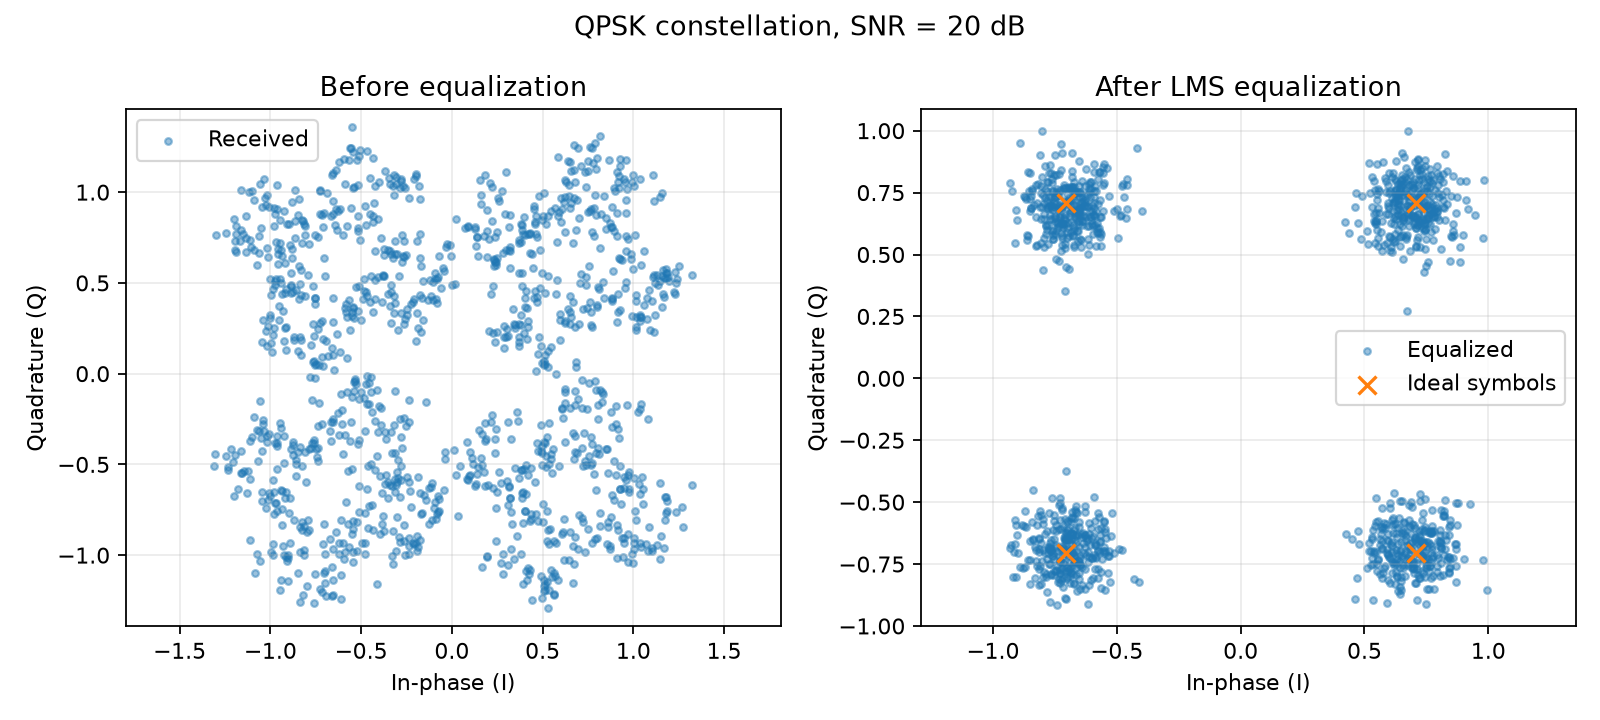
\includegraphics[width=0.98\columnwidth]{../results/constellation_comparison.png}
\caption{Received and equalized test constellations for the default QPSK example.}
\label{fig:constellation}
\end{figure}

\begin{figure}[t]
\centering
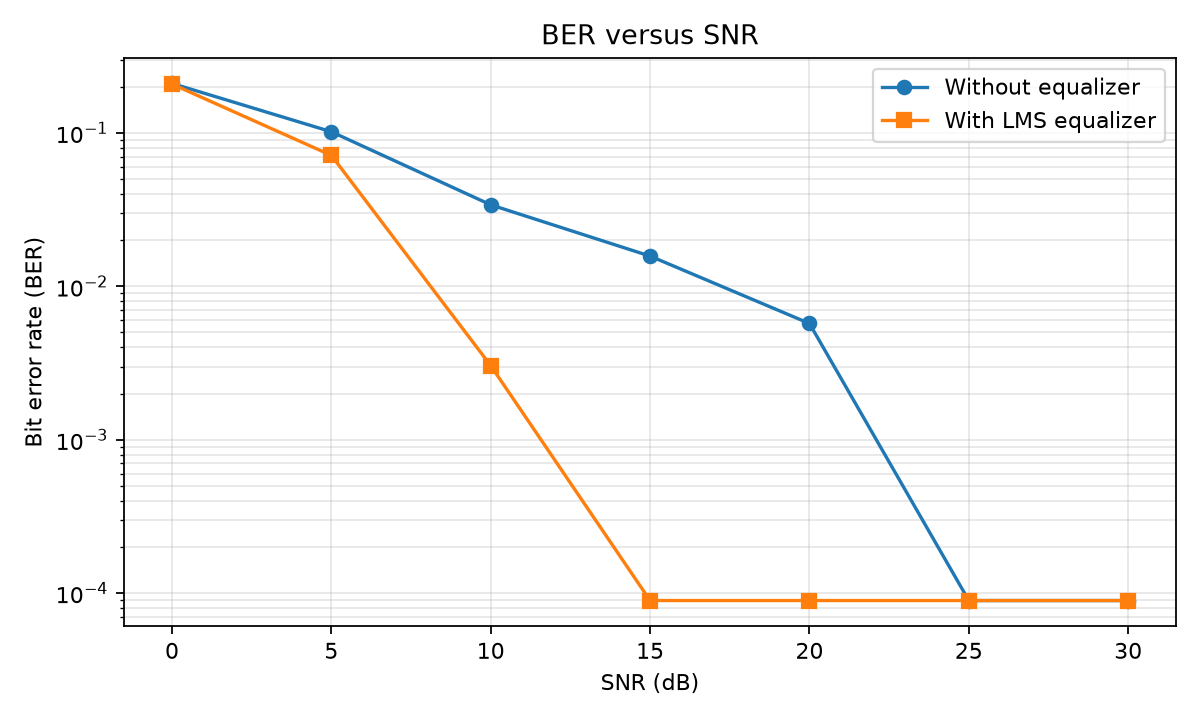
\includegraphics[width=0.98\columnwidth]{../results/ber_vs_snr.png}
\caption{Measured BER versus SNR. Describe the measurement count, finite-run limitations, and the trends actually observed.}
\label{fig:ber}
\end{figure}

% Discuss BER and EVM separately. Compare at least a few step sizes, tap
% lengths, modulation formats, or training lengths to satisfy the course brief.

\section{Conclusion and Limitations}
% State what the experiment demonstrates and what it does not demonstrate.
% This symbol-spaced model does not include timing recovery, carrier recovery,
% pulse shaping, or a hardware RF front end. Suggest one realistic next step.

\bibliographystyle{IEEEtran}
\bibliography{references}
\end{document}
